\chapter{High Level}
\label{High Level chapter}
\section{Overview}
This chapter explains the role of the High Level group in the whole system. The kidnapped robot problem is still quite an open issue in the robotics community and consequently the solution presented is quite conceptual. In order to solve the problem, our group decided to divide the kidnapping problem into two parts: detection of the kidnapping situation; and recovery after being kidnapped. Information sources available for these tasks consist of odometry data, laser data, hector\_mapping data, data from the Vision group and data from the Kalman group.

The structure of the whole system is shown in Figure \ref{System}. Section \ref{section:concept} gives out some basic ideas on how the kidnapping problem can be solved. Section \ref{section:relevant_ros_topics} lists the ROS topics that were used in the implementation. Section \ref{implementation} provides information on how the detection and recovery tasks were implemented. Section \ref{problems} describes the problems and difficulties met mainly during the testing process.

\begin{figure}[htb]
\centering
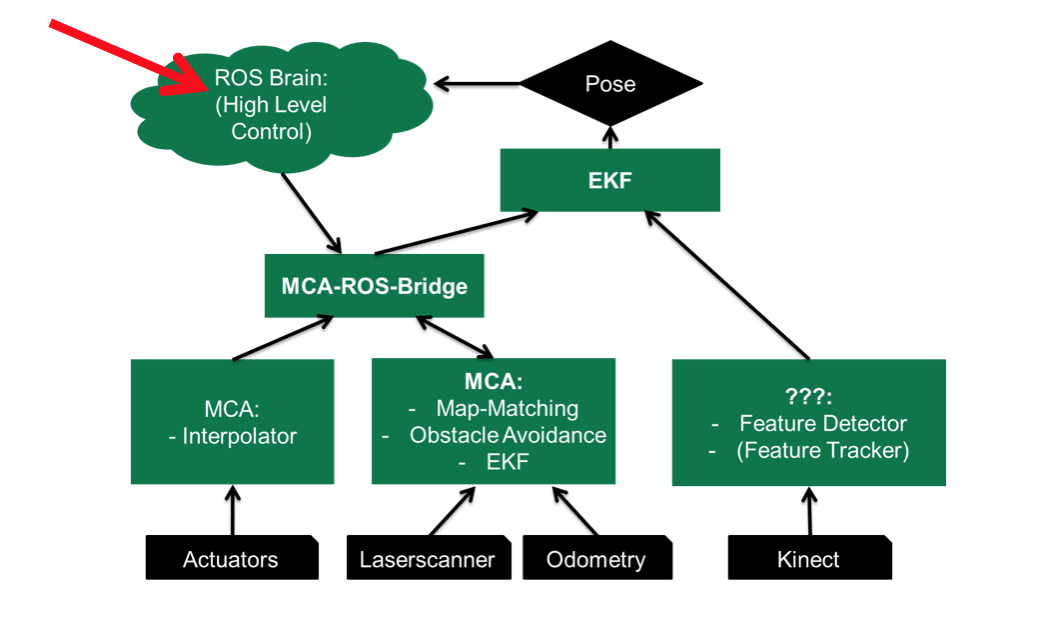
\includegraphics[width=0.9\textwidth]{graphics/system.png}
\caption{Overview of the system}
\label{System}
\centering
\end{figure}

\section{Concept} \label{section:concept}

\subsection{Kidnap Detection} \label{subsection:concept_detection}
There are several ways to detect a kidnapping situation. We could, for example, say that when one of our sensors are rendered unavailable, then there is a high chance that we are kidnapped at that point. We probably have to first determine which sensors are crucial for the localization. If there are redundant sensors in the system (i.e. there are 2 or more sensors that deliver similar data) then it would probably be fine if only one of them is available for the localization. We could also use some sort of passive landmarks to determine or check our current pose. The positions of the landmarks can be stored in the robot's database, so that the robot can do a lookup whenever it sees those landmarks. Another way to do the detection is to match the obtained obstacle point clouds with a map of the building that we have prepared beforehand. A low match rate could mean that we are not there, where we think we are. The list goes on, and will not be further discussed in this chapter.

For this task, we use 3 criteria to help detect the kidnapping situation. These criteria are: timestamp obtained from the sensor(s), QR markers, and the covariances of the pose obtained from the Kalman group. Further explanation will be given in the Subsection \ref{subsection:implementation_detection}. 

\subsection{Kidnap Recovery} \label{subsection:concept_recovery}

After being kidnapped, the robot should try to find out where it is currently located. There are several methods that help achieve that, e.g. Monte Carlo method, SLAM, Particle Filter, Kalman Filter. For this practical course, we have decided to use the Extended Kalman Filter to relocalize the robot.

In order to obtain new information after being kidnapped, our group proposes to use a maze-solving algorithm. The main idea of the algorithm is to explore the environment by going in one direction, e.g. forward, while always making sure that the obstacle is located nearby to one side of the robot. During the exploration, new data, such as: point clouds; landmarks; etc., can be obtained. These are then used to determine the robot's current pose. Detailed explanation regarding the implementation will be given in Subsection \ref{subsection:implementation_recovery}.





\section{Relevant ROS Topics}\label{section:relevant_ros_topics}

\subsection{Kidnap Detection}
The followings are the topics that were used and published by \texttt{kidnap\_detection}. The callbacks are done by using \texttt{ros::AsyncSpinner}, which allows parallel asynchronous callbacks to be performed.


\begin{description}
\item[List of subscribed topics]\
	\begin{itemize}
	\item  \textbf{``/kalman/fused\_pose''}: delivers the pose fused by the Kalman group. It is used by the robot to determine its current position.
	\item  \textbf{``/poseupdate''}: delivers the current pose data based on hector\_mapping. Its timestamp is the only thing that will be used by this node.
	\item  \textbf{``/vision/unexpected\_marker''}: if an unexpected marker is seen, \{\texttt{std\_msgs/Bool} data: True\} will be published to the topic.
	\item  \textbf{``/HL/is\_kidnapped''}: shows whether the robot is kidnapped. Kidnap detection will not be performed if the robot is currently kidnapped.
	\end{itemize}
\end{description}

\begin{description}
\item[List of published topics]\
	\begin{itemize}
	\item \textbf{``/HL/is\_kidnapped''}: the result of the kidnap detection will be published here.
	\end{itemize}
\end{description}

\subsection{Kidnap Recovery}

The followings are the topics that were used and published by \texttt{kidnap\_recovery}. The callbacks are done by using \texttt{ros::AsyncSpinner}, which allows parallel asynchronous callbacks to be performed.

\begin{description}
\item[List of subscribed topics]\
	\begin{itemize}
	\item \textbf{``/laser\_vor/scan''}: delivers the front laser scanner's data as \texttt{sensor\_msgs/LaserScan}. The laser data obtained from this topic will be mainly used to get the distance information of the obstacles located in front and to the left of the robot.
	\item \textbf{``/laser\_hinter/scan''}: delivers the back laser scanner's data as \texttt{sensor\_msgs/LaserScan}. The laser data obtained from this topic will be mainly used to support the laser data obtained from the front laser scanner.
	\item \textbf{``/HL/laser\_data\_obtained''}: indicates that data from one of the laser scanners have been obtained. This topic is used internally so that asynchronous callbacks can work correctly.
	\item \textbf{``/robot/lauron/odom''}: delivers the odometry data \texttt{nav\_msgs/Odometry}.
	\item \textbf{``/vision/sees\_marker''}: \{\texttt{std\_msgs/Bool} data: True\} will be published to the topic as long as the robot keeps seeing a QR marker. Used as an indicator to trigger some of the robot's behaviours (e.g. stopping).
	\item \textbf{``/vision/estimated\_pose''}: delivers the current pose of the robot on the global map, as was estimated by the Vision group. This pose will be deemed the most trustworthy by the robot and will be used, along with the current local pose of the robot, to calculate the transformation matrix needed to transform poses in the local map to the global map.
	\item \textbf{``/poseupdate''}: delivers the current pose data based on hector\_mapping. This pose represents the current pose of the robot in the local map, which will also be used, along with the estimated pose from the Vision group, to calculate the local to global map transformation matrix.
	\item \textbf{``/slam\_out\_pose''}: delivers the same pose information as the one we got from \texttt{/poseupdate}. The difference is that we do not get the covariance information from the topic.
	\item \textbf{``/HL/is\_kidnapped''}: if \{\texttt{std\_msgs/Bool} data: True\}, then the kidnap recovery procedure will be started. Otherwise, this node will just publish the last local to global /tf data that it has calculated.
	\end{itemize}
\end{description}

\begin{description}	
\item[List of published topics]\
	\begin{itemize}
	\item \textbf{``/robot/lauron/cmd\_vel''}: the desired \texttt{geometry\_msgs::Twist} of the robot will be published here.
	\item \textbf{``/HL/laser\_data\_obtained''}: \{\texttt{std\_msgs/Bool} data: True\} will be published, once data from one of the laser scanners have been obtained.
	\item \textbf{``/HL/is\_kidnapped''}: every time a marker is seen by the robot when it is kidnapped, \{\texttt{std\_msgs/Bool} data: False\} will be published.
	\item \textbf{``/vision/unexpected\_marker''}: once the robot has finished recovering itself, \{\texttt{std\_msgs/Bool} data: False\} will be published to this topic.
	\item \textbf{``/initialpose''}: this topic is currently not in use, and is currently commented out in the implementation due to lack of time to test the method. This can however be used to reset the pose of the robot to a desired local pose. It is mainly used because the pose obtained from \texttt{/poseupdate} is not reliable enough, in the case that some sensors are turned off or are malfunctioning. This can therefore be used to set the correct local pose obtained by inverse transforming the global fused pose from the Kalman group to the local pose.
	\item \textbf{``/tf''}: after the recovery procedure has been successfully performed, the transformation matrix that is used to transform local poses to the global map will be calculated and published to this topic.
	\end{itemize}
\end{description}

\section{Implementation}\label{implementation}

\subsection{Kidnap Detection}\label{subsection:implementation_detection} 
As mentioned before in Subsection \ref{subsection:concept_detection}, 3 criteria are used to detect kidnapping of the robot, e.g. timestamp of the sensor(s), QR marker, and fused pose from the Kalman group. 

\begin{enumerate}

\item \textbf{Timestamp of the Sensor(s)} \hfill \\
We used the timestamp obtained from \texttt{/poseupdate} as basis for our timestamp-based detection. We wanted to use the timestamp from the odometry, but apparently the topic \texttt{/robot/lauron/odom} keeps delivering data, even when the motors are turned off.

The timestamp is used to determine whether the sensors are still working as intended. This is done by comparing the current time of ROS with the last timestamp that we obtained from the sensor. If the difference between the two exceeds the defined threshold (in our case it is 2.0 seconds), then that would mean that something went wrong with (some of) the sensors, and thus the robot is now kidnapped.

\item \textbf{QR Marker} \hfill \\
The Vision group continuously decides which QR marker is to be expected based on the robot's current pose, which is the Kalman fused pose. Each time a QR marker is seen by the robot, the marker is compared to the next expected marker. If the markers do not match, then Vision group will publish \{\texttt{std\_msgs/Bool}: True\} to the  \texttt{/vision/unexpected\_marker} topic. Data with the value True from this topic will trigger a kidnapping event.

If a kidnapping situation is detected through this method, then the X- and Y-variances will be extracted from the pose covariances obtained from the Kalman group. These will then be stored and used as thresholds for the next ``Kalman Fused Pose'' detection. We assume that the covariances we got at this point to be ``high'', because the robot is now at a different location compared to what the Kalman group told the robot. The Z-rotation variance is not used, because it fluctuates way too much with a large difference.

\item \textbf{Kalman Fused Pose} \hfill \\
The robot constantly receives the current Kalman fused pose from the topic \texttt{/kalman/fused\_pose}. X- and Y-variances are extracted from the covariances from the fused pose, and are compared with the thresholds, which were set in the ``QR Marker'' detection phase. The thresholds are initialized to \texttt{Float.INFINITY}.

\end{enumerate}

The 3 detection criteria are performed inside ROS callbacks. This means that each time new data is published to their corresponding topics, the detection will be triggered. Additionally, all detections are also performed every 2 seconds, regardless whether there are new data or not. This is done in order to successfully detect the kidnapping situation, where all the sensors and localization nodes are turned off. Once a kidnapping event has been fired, no further detection will be performed until we obtain \{\texttt{std\_msgs/Bool} data:False\} from \texttt{/HL/is\_kidnapped}.

We read a lot of papers and publications about the problem and did a lot of brainstorming before we came to our solution. We thought that a ``big change'' in covariances, which could be obtained by calculating the second order derivation of the covariances, should be used to detect the kidnapping, instead of using the variances as they are. However, it is not clear how big of a difference in values is ``big'' in our situation.


\subsection{Kidnap Recovery} \label{subsection:implementation_recovery}

Whenever the Recoverer detects that its status has changed from being localized to being kidnapped, it will execute the kidnap recovery algorithm. As previously mentioned in Subsection \ref{subsection:concept_recovery}, the recovery algorithm is implemented based on maze-solving algorithms. The obstacles have to be located on the left of the robot in our implementation. We decided on this, because the front laser scanner is also located on the left side of the robot, which makes detecting obstacles while moving forward much easier.

The recovery or exploration algorithm is performed as follows: the robot first has to move towards the nearest obstacle and align itself parallelly to the obstacle, with the obstacle being on its left side. Afterwards, it moves forward until it detects a free space (room) on its left side, where it can go inside and start exploring, or an obstacle located at the front of the robot, to which the robot will align itself parallelly (obstacle will be located on its left side after rotating). While moving forward, the robot ensures at all times, that it is still aligned parallelly to the left obstacle. It also ensures that the distance to the left obstacle is large enough for a successful rotation. The robot will continue exploring until a QR marker (or other features) has been spotted. At the end, a transformation matrix, that describes how local poses of the robot can be transformed to the global map, is published to the \texttt{/tf} topic. This information will be used by the Kalman group to transform their local poses.

Safety measures are also implemented, so that the robot does not collide with obstacles during movement or rotation. For example, safety zones are defined for when the robot is moving forward, which can be seen in Figure \ref{Zone}.

The recovery algorithm is divided into two phases: preparation for the exploration and the exploration itself. Detailed explanation regarding how these are implemented will be given in the subsections below.

\subsubsection{Basic Movements and Functions}
Some of the basic movements (functions), that are going to be referenced later in Subsection \ref{subsection:implementation_preparation}, and Subsection \ref{subsection:implementation_exploration}, are described in the following list:




\begin{itemize}
\item \textbf{stopUntilStopped()}: \label{item:stopUntilStopped}
This function stops the robot completely. Stopping the robot is done by publishing \{0, 0, 0, 0, 0, 0\} twist to \texttt{/robot/lauron/cmd\_vel}. Solely publishing the twist would allow any actions that are performed after publishing the twist values to be executed directly afterwards, without waiting for the robot to be completely stopped. Which is why we implemented a waiting function that reads from the topic \texttt{/robot/lauron/odom} and does nothing until both values from the twist that is obtained from the topic approximates 0.


\begin{figure}[htb]
\centering
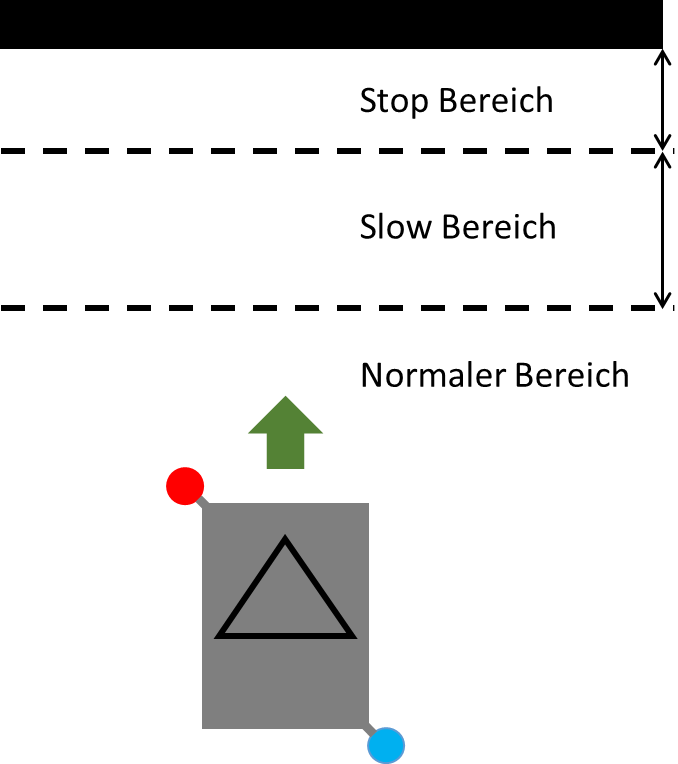
\includegraphics[scale=0.6]{graphics/Zone.png}
\caption{Various speed zones based on the distance to the obstacle}
\label{Zone}
\centering
\end{figure}


\item \textbf{goForward()}: \label{item:goForward}
This function sets the velocity of the robot in the x-direction of the ROS coordinate system with the pre-defined \texttt{DEFAULT\_FORWARD\_VELOCITY}. This function is used whenever the robot is located within the normal area, far away from the obstacles on the front (Figure \ref{Zone}).

\item \textbf{goSlower()}: \label{item:goSlower}
This function sets the velocity of the robot in the x-direction of the ROS coordinate system with the pre-defined \texttt{SLOW\_FORWARD\_VELOCITY}. This function is used whenever the robot is located within the slow area, so that the robot will be able to stop itself in time, to avoid collision with the front obstacle (Figure \ref{Zone}).


\item \textbf{rotate(Degree angleInDegree)}: \label{item:rotate}
This function allows the robot to rotate itself around its center with the given angle. the angular velocity is firstly determined according to the given rotation angle. If the rotation angle is larger than 5$^{\circ}$, the robot will stop any actions it was doing, and rotate itself with the \texttt{DEFAULT\_OMEGA\_IN\_DEGREE} angular velocity. Otherwise, the robot rotates itself with the slower angular velocity (\texttt{SLOW\_OMEGA\_IN\_DEGREE}). This is done so that small changes in angle do not interfere with other movements, such as goForward() (see \ref{item:goForward}). 

Before rotating itself, the robot stores its initial orientation (obtained through \texttt{``/slam\_out\_pose''}). During the rotation, the robot constantly compares the current orientation (obtained from \texttt{``/slam\_out\_pose''}) with the initial orientation. Once the robot has achieved the given rotation angle, the rotation is stopped. Do note that the orientation information we obtained from \texttt{``/slam\_out\_pose''} is absolute, which means that calculating the angle difference is not so trivial. The orientation information that we obtained also fluctuate slightly, which posed a problem at the beginning of the rotation (problem already solved).
\end{itemize}

\subsubsection{Exploration Preparation} \label{subsection:implementation_preparation}

Before the robot can start with the exploration, it has to do some preparation for it. Basically, the robot needs to move towards the nearest obstacle and align itself parallelly to it. The whole recovery algorithm is implemented in the \texttt{startRecovery()} function. Parts before the while()-loop belongs to the preparation part, and the rest belongs to the exploration part. The flow of the \texttt{startRecovery()} function is shown in Figure \ref{start_recovery}.

\begin{figure}[htb]
\centering
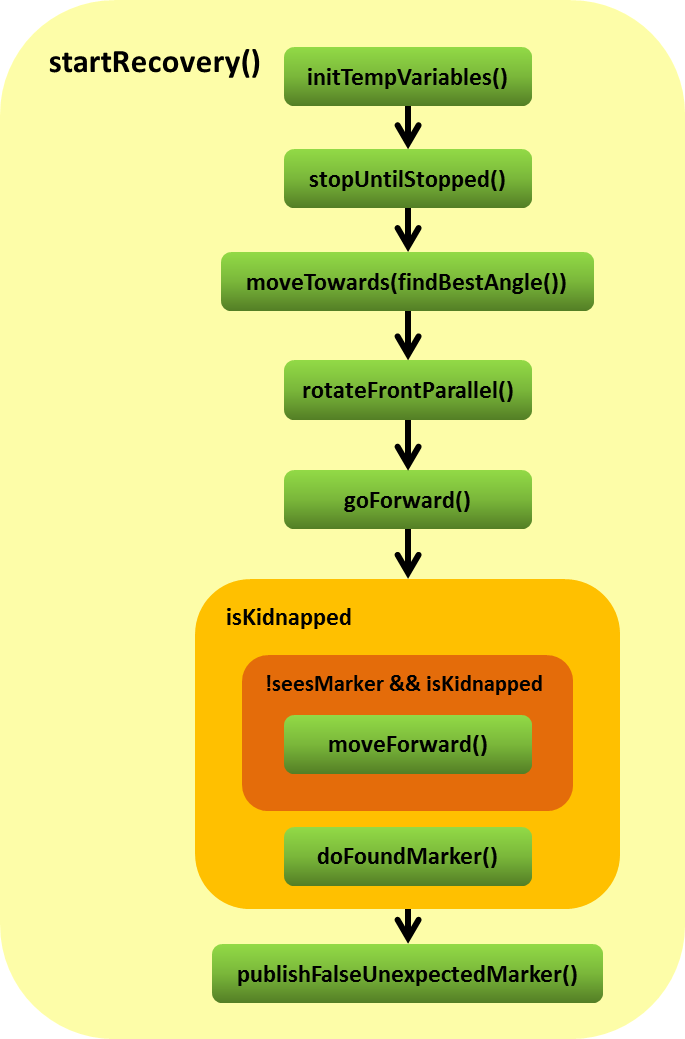
\includegraphics[scale=0.8]{graphics/start_recovery.png}
\caption{Recovery algorithm}
\label{start_recovery}
\centering
\end{figure}

\begin{description}
\item \textbf{initTempVariables()} \hfill \\
This function resets some of the attributes that could not be reset otherwise. For example, the attribute \texttt{seesMarker} will be reset to false. This function ensures that the startRecovery() function can be executed without any unexpected side effects.

\item \textbf{stopUntilStopped()} \hfill \\
(See \ref{item:stopUntilStopped})

\item \textbf{lookAround()} \hfill \\
This function causes the robot to make a full 360$^{\circ}$ rotation to observe the environment. The distance information (in meter) between the front laser scanner and the nearest obstacle located in front of it (Figure \ref{best}), along with the current absolute orientation angle of the robot are sampled and stored into a distance map every couple of seconds. The robot will stop after it has completed the full rotation.

\begin{figure}[htb]
\centering
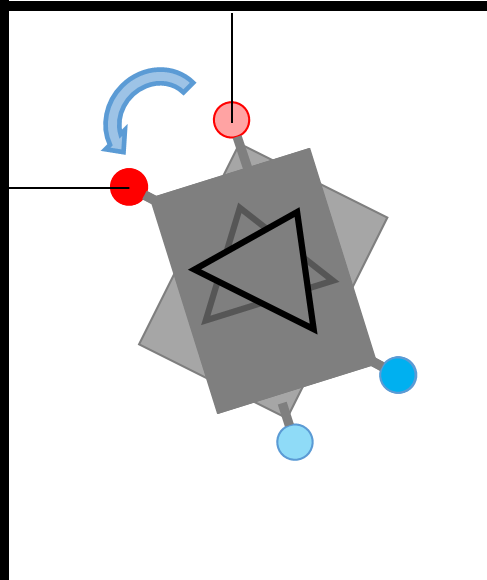
\includegraphics[scale=0.5]{graphics/find_best_angle.png}
\caption{Looking around}
\label{best}
\centering
\end{figure}


\item \textbf{findBestAngle()} \hfill \\
This function searches the distance map, that was initialized during lookAround(), and returns the absolute local angle in which the distance to the front laser scanner was the shortest. 

\item \textbf{moveTowards(findBestAngle())} \hfill \\
This function moves the robot towards the ``bestAngle''. First the robot has to do rotate(bestAngle) (see \ref{item:rotate}). Afterwards, it simply goes forward (goForward(), see \ref{item:goForward}), until it reaches the slow or stop zone (Figure \ref{Zone}).

\item \textbf{goForward()} \hfill \\
(See \ref{item:goForward}). This is done to ensure that the robot is moving forward before the actual exploration begins.
%Finding the best angle means simply calculating the minimum distance among sampled scans and returning its angle, as shown in Figure \ref{best}, now in millimeters. Due to laser properties negligibly small distances are not considered.
 
\begin{figure}[ht]
\centering
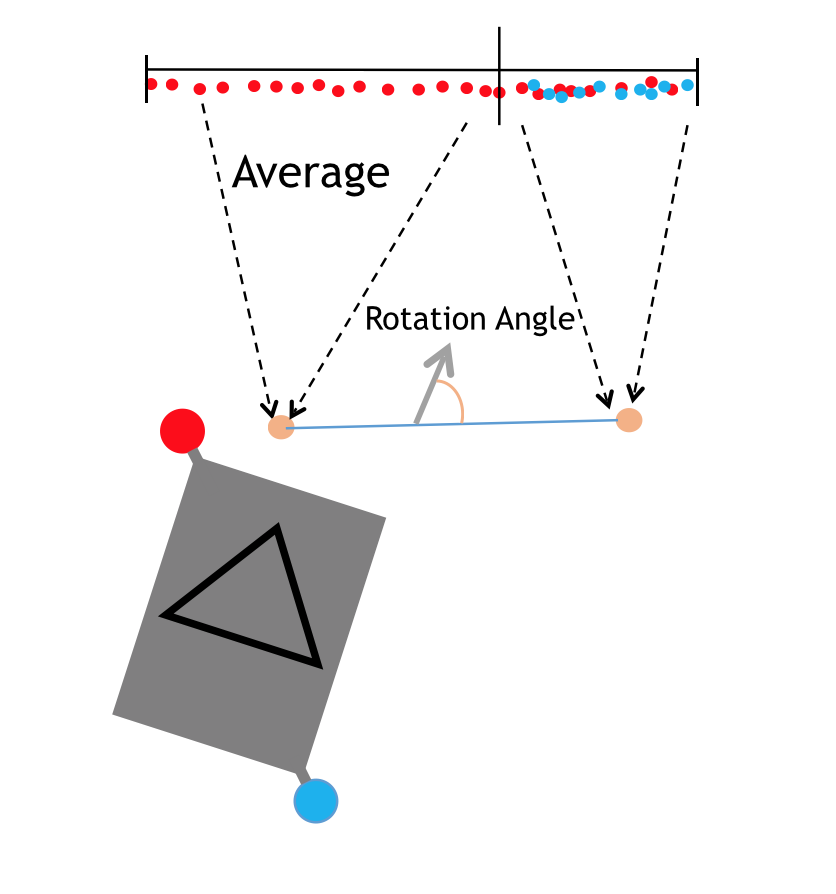
\includegraphics[scale=0.575]{graphics/front_parallel.png}
\caption{Calculating the front parallel rotation angle}
\label{parallel}
\centering
\end{figure} 
 
\item \textbf{rotateFrontParallel()} \hfill \\
This function rotates the robot until it is aligned parallelly to the front obstacle, with the obstacle being on the robot's left side after the rotation has been performed. As shown in Figure \ref{parallel}, merged data from both front and back laser scanners are used. The scanners first search for the 2 points that are located nearest to the robot. The average of these 2 points are then calculated and used as a pivot for the next operation. All the obstacle points located inside the relevant area (Figure \ref{betrachteter_bereich}) and inside the ``pivot.y +/- LASER\_ERROR\_DEVIATION'' area are separated into two groups, so that both groups would have more or less the same amount of obstacle points. An average point is then calculated from each group. The resulting final left and right average points form a vector, to which the robot has to align itself parallelly. The averaging adds robustness to the process.

\begin{figure}[htb]
\centering
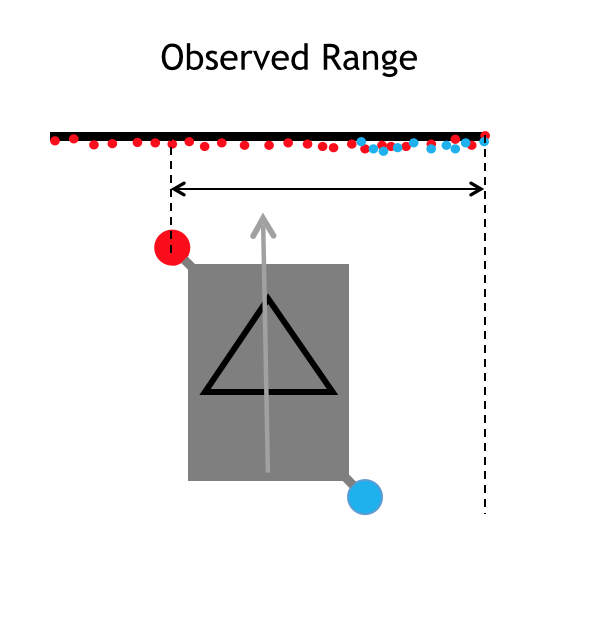
\includegraphics[scale=0.8]{graphics/betrachteter_bereich.png}
\caption{Relevant area for the front parallel rotation}
\label{betrachteter_bereich}
\centering
\end{figure}

Due to the fact that the robot rotates itself clockwise to do \texttt{rotateFrontParallel()}, the relevant front area of the robot is asymmetrical as shown in Figure \ref{betrachteter_bereich}. The left border of the area is influenced by the nearest left obstacle, meaning that when a left obstacle is located too near to the robot, the left border will be shifted to the left. This is done in order to obtain a correct front obstacle estimation vector.
\end{description}

\subsubsection{Exploration} \label{subsection:implementation_exploration}

After everything has been prepared, the robot can now begin with the exploration. The main part of the exploration is the \texttt{moveForward()} function in \texttt{startRecovery()} (Figure \ref{start_recovery}). The robot will keep moving forward as long as it is still kidnapped. At the end of the exploration, after it has found a marker, the transformation matrix between the \textbf{/local\_map} and \textbf{/global\_map} is updated and published to the \texttt{/tf} topic. A flowchart of how the \texttt{moveForward()} function is implemented, is shown in Figure \ref{move_forward}.

\begin{figure}[htb]
\centering
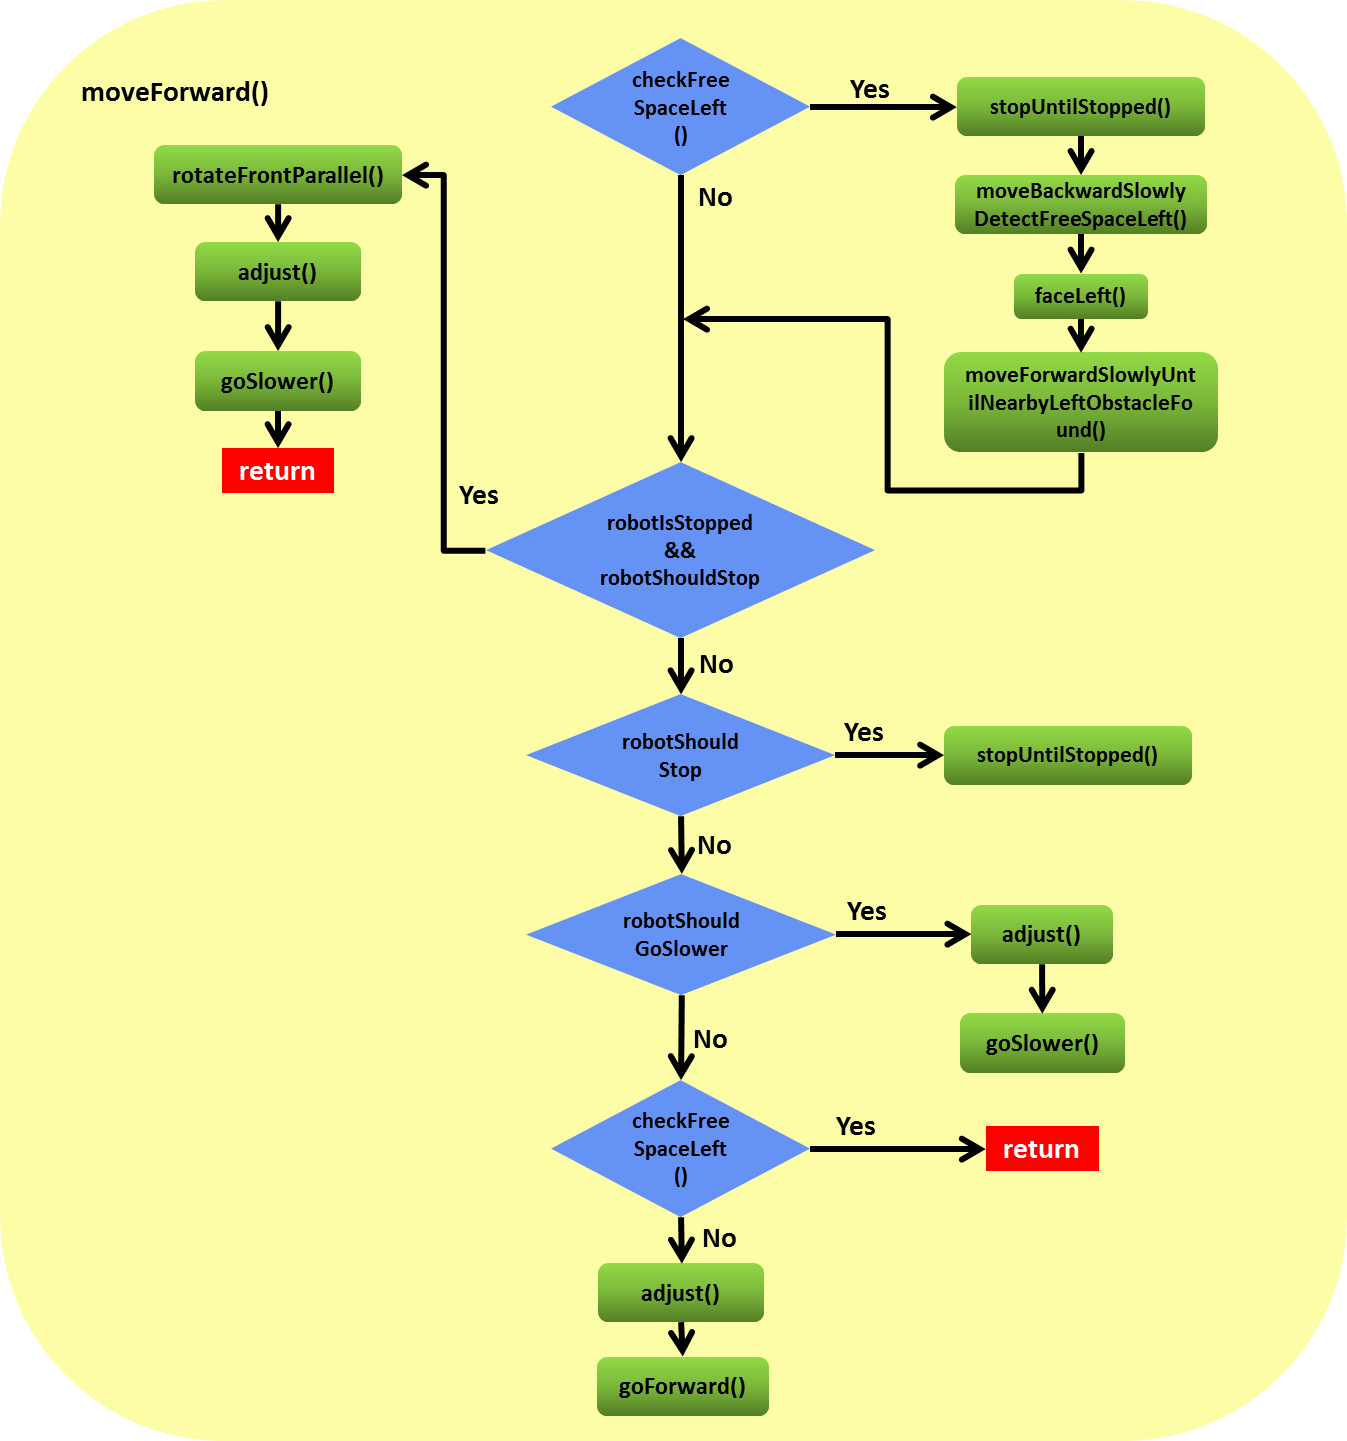
\includegraphics[width=0.9\textwidth]{graphics/move_forward.png}
\caption{Flowchart of moveForward()}
\label{move_forward}
\centering
\end{figure}

The following shows a list of attributes that are used during the exploration:

\begin{itemize}
\item \textbf{isKidnapped}:
Indicates whether the robot is currently being kidnapped or not. This attribute is updated through subscription to the ROS topic \texttt{/HL/is\_kidnapped}.

\item \textbf{seesMarker}:
Indicates whether the QR marker was seen by the Kinect camera. This attribute is updated through subscription to the ROS topic \texttt{/vision/sees\_marker}. This attribute is always reset to false each time startRecovery() is executed.

\item \textbf{robotIsStopped}:
Indicates whether the robot is stopped or not. Value for the attribute is obtained through comparing the current twist of the robot with the {0, 0, 0, 0, 0, 0} vector array.

\item \textbf{robotShouldGoSlower}:
 Indicates whether the robot should go slower. This is the case, if the current distance to the nearest front obstacle is between \texttt{MIN\_FRONT\_DISTANCE} (defined as 0.3 meter) and \texttt{MIN\_CAUTION\_DISTANCE} (defined as 0.11 meter).

\item \textbf{robotShouldStop}:
Indicates whether the robot should stop. This is the case, if the current distance to the closest front obstacle is shorter than \texttt{MIN\_CAUTION\_DISTANCE}  (defined as 0.11 meter).
\end{itemize}


The following describes how the rest of the functions in \texttt{startRecovery()} are implemented:
\begin{description}

\item \textbf{doFoundMarker()} \hfill \\
This function is executed every time a QR marker is seen. In order to constantly see the marker, the robot should stop its activities for a certain amount of time (it is currently defined as 0.5 seconds). Otherwise, it is possible that the marker could not be tracked or recognized correctly because of sudden movements, acceleration, or turning. Afterwards, the robot publishes \{\texttt{std\_msgs/Bool} data: False\} to \texttt{/HL/is\_kidnapped} to indicate that it is not kidnapped anymore.

\item \textbf{publishFalseUnexpectedMarker()} \hfill \\
This function is executed at the end of the exploration to indicate that the currently seen marker is not an unexpected marker. It publishes \{\texttt{std\_msgs/Bool} data: False\} to the topic \texttt{/vision/unexpected\_marker}.

\end{description}

The following describes how the functions in \texttt{moveForward()} are implemented:


\begin{description}

\item \textbf{checkFreeSpaceLeft()} \hfill \\
This function checks whether there is a free space on the left side of the robot. Free left space will only be detected if there is a left obstacle behind the robot. The robot should also be able to theoretically rotate itself 90$^{\circ}$, move forward, and fit at least 50\% of its body length without colliding with an obstacle, in order for it to be detected as a free space.

\item \textbf{moveBackwardSlowlyDetectFreeSpaceLeft()} \hfill \\
This function is used to make sure that the robot did not go too far ahead during the previous \texttt{checkFreeSpaceLeft()}, and that the free space it had detected was correct. The robot goes backward with \texttt{-SLOW\_BACKWARD\_VELOCITY} until free left space is detected and until the minimum time \texttt{BACKWARD\_PAUSE} has elapsed. The presence of the free space should remain if environment did not change.

\item \textbf{faceLeft()} \hfill \\
This function simply rotates the robot 90$^{\circ}$ counterclockwise so that the robot can go inside the free space it has detected.

\item \textbf{moveForwardSlowlyUntilNearbyLeftObstacleFound()} \hfill \\
This function ensures that the robot can go inside the free left space without colliding with an obstacle. In order to do that, the robot moves slowly forwards while trying to not collide with the left obstacle. This is done until a nearby left obstacle is detected around or behind the robot's center.

The function \texttt{checkObstacleLeftFrontBlindSpot()} ensures that the robot will not collide with the left obstacle. It checks for any obstacles located on the front left side of the robot. If there are obstacles closer than the pre-defined \texttt{FREE\_LEFT\_SPACE\_DISTANCE}, the robot rotates itself 4$^{\circ}$ clockwise to steer away from the obstacle, otherwise it rotates itself 8$^{\circ}$ counterclockwise to find the obstacle. This solution prevents a situation in which the robot moves on without noticing an obstacle in its blind spot.

\item \textbf{rotateLeftParallel()} \label{item:rotateLeftParallel} \hfill \\
This function ensures that the robot is aligned parallely to the left obstacle. Only obstacle points from the front laser scanner are used in this function (Figure \ref{rotate_left_parallel01}). The rotation angle needed for the parallel rotation can be obtained by measuring the angle between the normal of the robot with the the vector shown in Figure \ref{rotate_left_parallel02}. In order to obtain the vector, the scanner first search for the 2 points that are located nearest to the robot. The average of these 2 points are then calculated and used as a pivot for the next operation. All the obstacle points located between the robot's length (+ some small distance to the front) and inside the ``pivot.x +/- LASER\_ERROR\_DEVIATION'' area are separated into two groups, so that both groups would have more or less the same amount of obstacle points. An average point is then calculated from each group. The resulting final left and right average points form the vector for the angle calculation. Points located too far away from the pivot will not be considered, because otherwise, the rotation angle will not reflect the actual obstacle and may lead to collision with the left obstace.

\item \textbf{adjustLeftDistance()} \label{item:adjustLeftDistance} \hfill \\
This function ensures that the robot maintains a proper distance to the left obstacle. The distance has to be wide enough to rotate successfully, but not too wide since our implementation of the maze-solving algorithm requires the robot to keep moving along the left obstacle. The reasonable range is defined as [\texttt{MIN\_ROBOT\_LEFT\_DISTANCE\_INTERVAL}, \texttt{MAX\_ROBOT\_LEFT\_DISTANCE\_INTERVAL}]. Normally, the robot will be able to adjust its distance without affecting the linear x-velocity. However, if the distance to the left obstacle is too too large, the robot will stop moving forward, so that no side effects may occur. When the robot moves to right direction, the function \texttt{checkRightObstacle()} is executed to check whether moving to the right direction would result in a collision or not. 

\item \textbf{adjust()} \hfill \\
This function adjusts the robot's pose in respect to the left obstacle by doing \texttt{rotateLeftParallel()} (see \ref{item:rotateLeftParallel}) and \\ \texttt{adjustLeftDistance()} (see \ref{item:adjustLeftDistance}).

\begin{figure}[ht]
\centering
\begin{subfigure}{.5\textwidth}
	\centering
	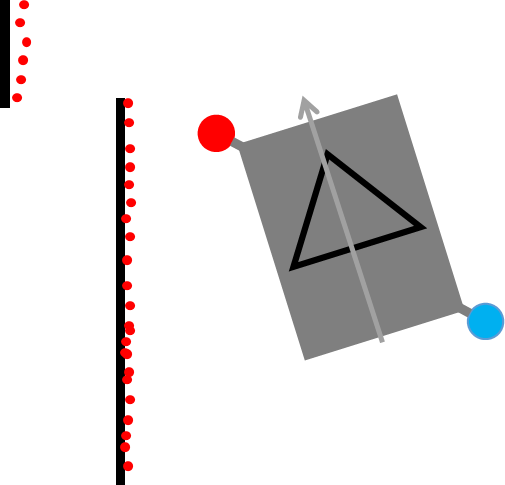
\includegraphics[scale=0.65]{graphics/rotate_left_parallel01.png}
	\caption{Point clouds of the left obstacles obtained from the front laser scanner}
	\label{rotate_left_parallel01}
\end{subfigure}%
\begin{subfigure}{.5\textwidth}
	\centering
	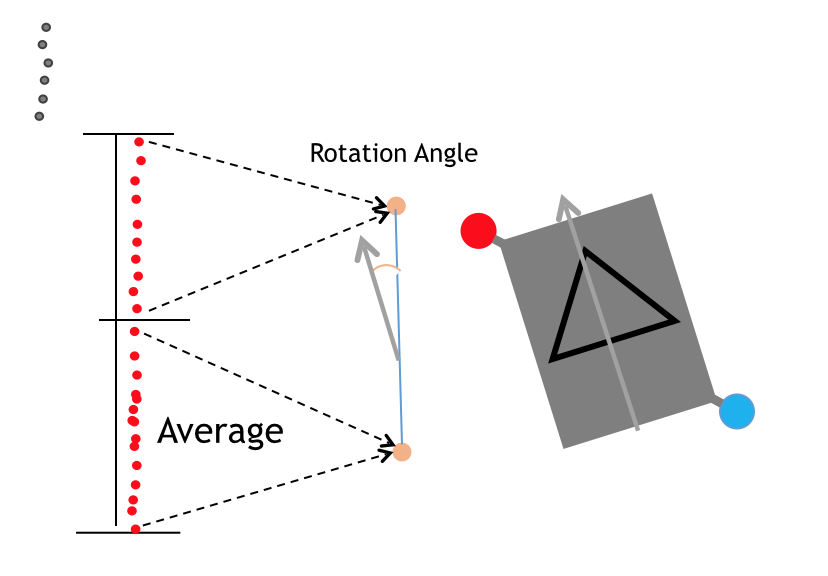
\includegraphics[scale=0.55]{graphics/rotate_left_parallel02.png}
	\caption{Finding the correct rotation angle}
	\label{rotate_left_parallel02}
\end{subfigure}
\caption{rotateLeftParallel()}
\label{fig:side_by_side}
\end{figure}

\item \textbf{goSlower()} \hfill \\
(See \ref{item:goSlower}.) 
\end{description}



\section{Problems and Difficulties} \label{problems}
During the course of the practical course, we encountered several difficulties during implementation and testing. These are listed in the following subsections.

\subsection{Testing on Simulator}

There was a time when we thought that we wanted to test our recovery algorithm on the MCA simulator, because the robot was not available at the time. Setting up the simulator was not so simple and took a lot of time due to the lack of documentation. We had to get help from Marc to successfully set the simulator up, which still took quite some time to find the correct commit. However, the problem did not stop there. The ROS-MCA interface has not been fully implemented yet at the time, so we thought we would use this time to get to know MCA2 better and to prepare our code for the simulator. After the ROS-MCA interface has been implemented, we adjusted our code to make it functional. We tried testing it out afterwards, but sadly it still did not work. The problem was because the laser scanners keep giving us data, as if the obstacles are not there. So we had to wait for the solution while finding out what the problem was in the meantime by ourselves. We had to modify the configuration file (angle of x-axis, min angle, max angle, position) for the laser scanners on the simulator as well, because it did not represent the laser scanners on pfosten. Finding which configuration file we need to change was also a challenge, because of the lack of documentation. 

At some point, we managed to get the MCA2 to work perfectly. However, we still see some strange things happening on the simulator. Again, we took a lot of time to solve this issue. We thought that the problem lied on our code, but it turns out that the twists that we published are somehow interpreted as global twists for the robot. Meaning that no matter how the robot is oriented in the global map, when the linear x velocity for the robot is set, then the robot will move along the x-axis of the global map. We had to fix this as well, and finding the correct mca file, we needed to change, also took quite some time.

At the end, our recovery algorithm works more or less on the simulator, which was caused by the error model that was implemented in the MCA2 module. There are some improvements to be made, but it could be seen that it was going on the right track. Then comes the testing with the real robot. The algorithm performed on the robot did not even come close to the achieving the same results we obtained from the simulation. We had to change a lot of things in order for it to work on the robot.

Long story short, we wasted a lot of time on the simulator.


\subsection{Calibration}

Even after we have changed and improved our implementation, some of our functions still could not work properly. We only noticed it after comparing the raw laser scanner data obtained from the two laser scanners, and found out that the data did not really match one another. Later we found out that we could have achieved the same result by using rviz.

The two laser scanners of the robot turned out to not have been calibrated properly. Due to the lack of documentation, it was especially hard to find the correct configuration files for the laser scanners. We spent a big amount of time searching for the correct configuration file by changing the parameter values and observing the results in rviz. After finding the correct files, we now have to accurately measure the positions of the laser scanners and adjust it accordingly in the configuration files. We were told specifically not to modify the laser scanners physically. So we had to measure angle differences manually.

Measuring the angle differences manually was a really meticulous task. We had to first find out what points are considered the minimum and maximum range of the laser scanner. Then we had to align large straight objects to the robot, and calculate the angle difference between the object and the extreme points. Afterwards, these values are written into the configuration files and are tested on rviz. We wanted high precision on the data, so we tried to make both point clouds to completely overlap with one another. This however turned out to be impossible, so we had to determine which regions should overlap the most. We tried testing our algorithm afterwards, and it worked.

Some time afterwards, we tried testing our algorithm again, and it did not work. Turned out that the lasers have to be re-calibrated. So we decided not to do the same calibration method that we did before, due to the long time it consumed. We found out that both laser scanners actually have the same min and max angle (from the center of the laser scanner), and that both encompass the same area. So we decided to tweak the configuration data again to emulate this behaviour. Afterwards, we physically rotated the laser scanners in order for them to cover the areas they were supposed to cover. After we have confirmed that they are now correctly calibrated, we marked the laser scanners with a pencil, so that the next time we need to calibrate them again, we would be able to do so more easily with the help of a T square ruler. 

\subsection{WLAN}

The WLAN was the biggest annoyance we encountered during the robot testing phase. Before all the data were transferred to the robot's system, we had to use WLAN to communicate with the ROS topics. Sometimes the WLAN works so slowly, that data were not exchanged correctly and thus lead to false test results.

\subsection{Floor Level}

In HoLL there is an inclined plane in the middle of the corridor. Since the laser sensors operate on one specific height, at a certain point, some parts of the inclined plane were detected as an obstacle, just the same as any wall around. To avoid this, proper interpretation of the distance measure had to be considered. However, the real problem with the floor level, is that it is not possible to detect the lack of obstacles caused by the difference in height. For example, it is impossible for the robot to say whether it can move towards the edge of the inclined plane (that is not connected to the wall) without falling.

Another problem is that, when the robot was moving downwards and was instructed to stop, its wheels could not stop completely at once because it was actually coasting for some time.

\subsection{Uneven Surface}

Another difficulty for both the robot and for us was the uneven surface. Being on top of these surfaces would lead to incorrect odometry poses as well as incorrect movement or rotation results, due to the wheels' uneven contact to the surface. In the worst case, the wheels would spin in the air. Information from the odometry would then not reflect the reality anymore. Furthermore, due to this situation we often encountered situations, in which the robot tried to move to the right (or left) and it moved backwards instead. Because of the wrong movement direction, it is possible that the next obstacles information it obtained could result in an undesired behavior.

\subsection{Transparent Window}

The transparent office windows in HoLL also posed a difficulty. The laser sensors could not recognize the windows correctly and delivered point clouds not precise to the position of the windows. To solve this problem we used styrofoams and cardboards which we found in the laboratory to cover the windows and build provisional walls so that the laser sensors could detect them correctly.

% "several basic movements are firstly defined for the robot. Based on these basic functions, the robot can rotate itself to observe the obstacles around and prepares for the QR mark searching. It moves to the closest obstacle and adjust itself parallel to the obstacle. Then, the robot starts the exploration process." in outlook



